\documentclass[11pt,openany]{book}

\usepackage[T1]{fontenc}
\usepackage[utf8]{inputenc}
\usepackage{lmodern}
\usepackage{microtype}
\usepackage[margin=1in]{geometry}
\usepackage{amsmath,amssymb,amsthm,mathtools,mathrsfs}
\usepackage{booktabs,longtable,array,tabularx}
\usepackage{graphicx}
\usepackage{enumitem}
\usepackage{xcolor}
\usepackage{url}
\usepackage{hyperref}
\usepackage[nameinlink,noabbrev]{cleveref}
\usepackage{listings}
\usepackage{fancyhdr}
\usepackage{caption}

\definecolor{darkblue}{RGB}{20,55,100}
\definecolor{darkgreen}{RGB}{20,90,55}
\definecolor{darkred}{RGB}{125,35,35}
\hypersetup{
  colorlinks=true,
  linkcolor=darkblue,
  citecolor=darkgreen,
  urlcolor=darkred,
  pdftitle={Shape, Divisibility, and Stein Geometry of the Fabius--Rvachev Law},
  pdfauthor={Research report prepared for Vladimir Reshetnikov}
}

\graphicspath{{numerical_output/}}
\setlength{\parindent}{1.2em}
\setlength{\parskip}{0.2em}
\setcounter{tocdepth}{2}
\setcounter{secnumdepth}{3}
\sloppy

\pagestyle{fancy}
\fancyhf{}
\fancyhead[LE,RO]{\thepage}
\fancyhead[LO]{\nouppercase{\rightmark}}
\fancyhead[RE]{\nouppercase{\leftmark}}
\renewcommand{\headrulewidth}{0.4pt}
\setlength{\headheight}{14pt}

\newtheorem{theorem}{Theorem}[chapter]
\newtheorem{proposition}[theorem]{Proposition}
\newtheorem{lemma}[theorem]{Lemma}
\newtheorem{corollary}[theorem]{Corollary}
\newtheorem{conjecture}[theorem]{Conjecture}
\newtheorem{problem}[theorem]{Problem}
\theoremstyle{definition}
\newtheorem{definition}[theorem]{Definition}
\newtheorem{remark}[theorem]{Remark}
\newtheorem{example}[theorem]{Example}

\DeclareMathOperator{\supp}{supp}
\DeclareMathOperator{\Var}{Var}
\DeclareMathOperator{\Cov}{Cov}
\DeclareMathOperator{\ord}{ord}
\DeclareMathOperator{\Li}{Li}
\newcommand{\Up}{\operatorname{up}}
\newcommand{\sinc}{\operatorname{sinc}}
\newcommand{\E}{\mathbb{E}}
\newcommand{\Pp}{\mathbb{P}}
\newcommand{\R}{\mathbb{R}}
\newcommand{\C}{\mathbb{C}}
\newcommand{\N}{\mathbb{N}}
\newcommand{\dd}{\,\mathrm{d}}
\newcommand{\repo}{\textsc{ProveIt}}
\newcommand{\Imported}{\textcolor{darkblue}{\textsc{Imported}}}
\newcommand{\ProvedHere}{\textcolor{darkgreen}{\textsc{Proved here}}}
\newcommand{\Conjectural}{\textcolor{darkred}{\textsc{Conjectural}}}
\newcommand{\Status}[1]{\par\smallskip\noindent\textbf{Status:} #1.\par\smallskip}

\lstset{
  basicstyle=\ttfamily\small,
  frame=single,
  breaklines=true,
  columns=fullflexible,
  showstringspaces=false
}

\title{\Huge Shape, Divisibility, and Stein Geometry\\[0.4em]
       \Large of the Fabius--Rvachev Law\\[1em]
       \large Repository-Distinct Frontier Results, Conjectures,\\
       and a Formalization Program}
\author{Research report prepared for Vladimir Reshetnikov}
\date{August 30, 2026}

\begin{document}
\frontmatter
\maketitle

\chapter*{Abstract}
\addcontentsline{toc}{chapter}{Abstract}
The Fabius function, the Rvachev up-function, the Prouhet--Thue--Morse sequence,
geometric infinite sinc products, and the associated $q$-series form a remarkably
rigid dyadic system.  The accompanying repository already contains an unusually
large body of work on endpoint asymptotics, Lambert--$W$ carriers, dyadic arithmetic,
$q$-binomial acceleration, Bell--Bernoulli moment calculus, Fourier decay,
representation theory, inverse-function asymptotics, Legendre and Lagrange loops,
and formalization.  The purpose of this report is therefore not to repeat that
material, but to locate directions that remain genuinely absent from the audited
corpus and to push them far enough to yield complete theorems.

The first main result settles the critical binary endpoint of a strict
log-concavity conjecture stated in the repository.  The Rvachev density is already
known there to be log-concave.  Combining this with its nowhere-analyticity proves
that it is in fact \emph{strictly} log-concave on $(-1,1)$.  This is an unusual
strictly log-concave law: every derivative of the density and of its logarithm
vanishes at the mode.  The theorem yields strict log-concavity of the Fabius
cumulative distribution and survival functions, strict monotonicity of the hazard
and reverse hazard, a strict monotone-likelihood-ratio property, and strict
log-convexity of the derivative of the inverse Fabius function.  The refinement
equation then turns the increasing score into an explicit dyadic ratio inequality.

The second main result is a convolution-divisibility obstruction.  The entire
Fourier transform has simple zeros at every odd integer.  Consequently the
Rvachev probability law has no nontrivial identical convolution root of any order,
even though it is an infinite convolution of unequal uniform laws.  The same
argument applies to the full geometrically scaled uniform family.

The third main contribution develops the canonical Stein kernel of the centered
Fabius--Rvachev distribution.  We obtain exact Fabius-tail and conditional-moment
representations, exact values $\tau(0)=5/36$ and $\tau(1/2)=1/12$, a moment bridge
to the repository's Bell--Bernoulli calculus, a weighted Poincare inequality with
sharp spectral gap one, and a symmetric diffusion generator having the Rvachev
law as invariant measure.  The Stein kernel is nowhere analytic, but its complete
Taylor jet at the mode is the quadratic $5/36-x^2/2$.  Therefore the formal
eigenvalue equation of the diffusion is exactly a rescaled Legendre equation.
This produces a new ``Legendre shadow'': smooth eigenfunctions have Legendre
Taylor jets, while global nonanalyticity rules out every analytic or polynomial
eigenfunction beyond the constants and the linear eigenfunction.

Finally, an exact logarithmic-coordinate representation and rigorous endpoint
bounds are derived for the Stein kernel.  They lead to a Lambert--$W$-compatible
asymptotic conjecture
\[
 \tau(1-\delta)\sim \frac{\delta}{1+\delta F'(\delta)/F(\delta)}
 \qquad (\delta\downarrow0),
\]
and to a program involving multiplicative concavity, factor-divisor rigidity,
Stein spectral asymptotics, strict log-concavity for the nonbinary family, and
Lean formalization.  A fully commented Python program and reproducible numerical
certificates accompany the report.

\chapter*{Research-status convention}
\addcontentsline{toc}{chapter}{Research-status convention}
Every substantial statement is marked according to the following convention.

\begin{center}
\begin{tabularx}{0.92\textwidth}{>{\bfseries}l X}
\toprule
\Imported & A fact proved in the repository or in cited literature and used here as input.\\
\ProvedHere & A complete proof is supplied in this report; the result was not found in the audited repository corpus.\\
\Conjectural & A precise but unproved statement, normally accompanied by structural or numerical evidence.\\
\bottomrule
\end{tabularx}
\end{center}

``Repository-distinct'' is intentionally weaker than a claim of absolute priority
in the global literature.  The searches were designed first to prevent duplication
of the supplied corpus.  The report does not assert that every proved-here theorem
has never appeared elsewhere under different terminology.

\tableofcontents
\listoffigures

\mainmatter

\chapter{Orientation and principal results}

\section{Why a new direction was necessary}
The repository has grown into a research library rather than a single article.
Its current top-level documentation contains a primary exposition, a mathematical
glossary, a non-elementarity study, a Lean walkthrough, an archive of historical
sources, a paper library, and both non-formalized and semi-formalized frontier
directories.  The semi-formalized draft manifest records large consolidated
volumes on Fourier decay, the Thue--Morse sequence, exponent sequences and
$q$-series, Lambert $W$, spectra and arithmetic, integration and transforms,
inverse functions and sampling, representations, exact polynomial synthesis,
and recent Lagrange--Legendre--Rvachev loops \cite{repo,manifest}.

That breadth invalidates several initially tempting claims of novelty.  In
particular, the following were explicitly discarded after collision checks.

\begin{longtable}{p{0.27\textwidth}p{0.63\textwidth}}
\toprule
Candidate direction & Reason for exclusion from the new-results list\\
\midrule
\endfirsthead
\toprule
Candidate direction & Reason for exclusion from the new-results list\\
\midrule
\endhead
Non-holonomicity of the sinc product and non-$P$-recursiveness of moments & Already proved in the consolidated Representation Frontiers volume.\\
General log-concavity and the plateau transition for geometric atomic densities & Already proved in the Exponent-Sequence and $q$-Series Frontiers volume.  Only the strict binary endpoint remained conjectural.\\
Fractional integration and complex-order transforms & Already treated at length in Integration and Transform Frontiers.\\
Fourier-shell asymptotics and log-periodic decay profiles & Covered by eight source reports and two comparative audits.\\
Legendre and Lagrange synthesis loops & The manifest records multiple dedicated reports, exact coefficient certificates, and consolidation work.\\
Bell--Bernoulli moment formulas and Lambert-series cumulants & Already part of the canonical $q$-series and arithmetic calculus.\\
\bottomrule
\end{longtable}

The viable gap was a probability-shape theory centered on \emph{strictness},
convolution roots, Stein kernels, and the diffusion naturally generated by the
Rvachev law.  None of the audited master volumes contains a Stein-kernel section,
and searches for ``Stein kernel'' and ``convolution root'' returned no relevant
repository result.  Strict log-concavity at the critical binary point is explicitly
left as a conjectural endpoint in the geometric-family treatment.

\section{Executive theorem map}
The report proves the following chain.

\begin{enumerate}[label=\textbf{R\arabic*.},leftmargin=3.2em]
\item The Rvachev density $p=\Up$ is strictly log-concave on $(-1,1)$.
\item The Fabius CDF and survival function are strictly log-concave; the hazard is strictly increasing, the reverse hazard strictly decreasing, and the location family has strict monotone likelihood ratio.
\item The derivative of the inverse Fabius function is strictly log-convex, although its complete nonconstant Taylor jet vanishes at probability $1/2$.
\item The score of $p$ equals the Fabius hazard and has the exact dyadic form
\[
 -\frac{p'(x)}{p(x)}=\frac{2p(2x-1)}{p(x)},\qquad 0<x<1.
\]
It rises strictly from $0$ to $+\infty$ and equals $4$ at $x=1/2$.
\item The Rvachev law has no $r$th identical convolution root for any integer $r\ge2$.
\item The canonical Stein kernel
\[
 \tau(x)=\frac{1}{p(x)}\int_x^1 t p(t)\,dt
\]
has exact Fabius-tail and conditional-residual-life forms, exact rational values,
and Bell--Bernoulli weighted moments.
\item The operator
\[
 \mathcal L g=\tau g''-xg'=\frac1p(\tau p g')'
\]
is symmetric in $L^2(p)$ and has exact weighted spectral gap $1$.
\item The Stein kernel is nowhere analytic, has formal center germ
$5/36-x^2/2$, and induces an exact Legendre equation on eigenfunction jets.
The only analytic eigenfunctions are $1$ and $x$.
\item An exact endpoint integral in logarithmic coordinates gives rigorous bounds
and a natural Lambert--$W$-scale asymptotic conjecture for $\tau(1-\delta)$.
\end{enumerate}

\section{A compact notation table}
\begin{center}
\begin{tabularx}{0.94\textwidth}{l X}
\toprule
Symbol & Meaning\\
\midrule
$U_n$ & independent $\operatorname{Unif}[0,1]$ random variables\\
$X$ & $\sum_{n\ge0}2^{-n-1}U_n$, the Fabius random variable\\
$F$ & CDF of $X$ on $[0,1]$\\
$V_n$ & $2U_n-1$, independent $\operatorname{Unif}[-1,1]$ variables\\
$Z$ & $2X-1=\sum_{n\ge0}2^{-n-1}V_n$\\
$p$ & density of $Z$, equal to the Rvachev up-function $\Up$\\
$H$ & CDF of $Z$\\
$I$ & inverse Fabius function $F^{-1}$\\
$Q$ & centered quantile $H^{-1}=2I-1$\\
$\tau$ & canonical Stein kernel of $Z$\\
$\rho(\delta)$ & endpoint elasticity $\delta F'(\delta)/F(\delta)$\\
$\sinc z$ & $\sin z/z$, with $\sinc 0=1$\\
\bottomrule
\end{tabularx}
\end{center}

\chapter{Corpus audit and nonduplication method}

\section{Inventory strategy}
The requested directory contains both active documents and historical snapshots.
A literal file count by itself is not a reliable duplication audit because many
old sources were later merged verbatim into canonical volumes.  The audit therefore
used three layers.

\begin{enumerate}
\item The top-level tree and all directory manifests were used to enumerate the
primary exposition, archive families, paper folders, Lean material, and frontier
groups.
\item Current canonical and consolidated LaTeX masters were read as the controlling
mathematical state of the project.  These include the primary Fabius--Rvachev
exposition and the master volumes for exponents and $q$-series, representations,
integration and transforms, inverse and sampling, spectra and arithmetic,
Thue--Morse formulas, and the recent polynomial/Legendre/Lagrange reports.
\item The archive README files and provenance notes were used to map superseded
LaTeX sources to the master documents into which they were absorbed.  Collision
searches were then run on the exact concepts needed here: strict log-concavity,
Stein kernels, convolution roots, weighted Poincare inequalities, diffusion
generators, and Legendre jets.
\end{enumerate}

This method reads the corpus according to its own editorial architecture.  A
historical file described as a verbatim predecessor of a consolidated volume was
not treated as a mathematically independent current source.  Conversely, recent
incoming reports not yet merged were checked separately because their distinctive
strands can be absent from the master volume.

\section{Imported facts used in this report}
Only a small portion of the repository's established theory is needed as input.
The imported statements are:

\begin{enumerate}
\item $p=\Up$ is the positive $C^\infty$ density of $Z$ on $(-1,1)$, vanishes
with all derivatives at $\pm1$, is even, and satisfies the refinement equation.
\item $p$ is log-concave on $(-1,1)$.
\item $p$ is nowhere real analytic on $[-1,1]$; in particular it is analytic on
no nonempty open subinterval of $(-1,1)$.
\item $F$ and $p$ take rational values at dyadic arguments, and the integration
volumes provide exact dyadic antiderivative algorithms.
\item The Fourier transform has the geometric sinc product and integer zero
divisor described below.
\item The centered even moments are generated by explicit Bernoulli cumulants
and complete Bell polynomials.
\item The endpoint and inverse-endpoint volumes provide all-orders expansions
whose scale selection is governed by Lambert $W$ and bounded dyadic-periodic
corrections.
\end{enumerate}

All new theorems below are derived from these inputs and standard named results
that are cited explicitly.

\section{External literature boundary}
The probability arguments use two classical tools.  First, convolution and
marginalization preserve log-concavity by the Prekopa theorem; modern surveys are
\cite{samworth,saumardwellner}.  Second, a one-dimensional density with connected
support has the canonical Stein kernel used below, and Saumard's weighted Poincare
inequality applies to it \cite{saumard}.  These tools are general; the exact
Rvachev formulas, dyadic identities, and Legendre consequences developed here do
not appear in those references.

\chapter{The dyadic probability fixed point}

\section{Random-series and refinement descriptions}
Let $(U_n)_{n\ge0}$ be independent random variables uniformly distributed on
$[0,1]$, and define
\begin{equation}\label{eq:Xseries}
 X=\sum_{n=0}^{\infty}\frac{U_n}{2^{n+1}}.
\end{equation}
The series converges almost surely and takes values in $[0,1]$.  Its CDF is the
Fabius function $F$.  Centering and doubling gives
\begin{equation}\label{eq:Zseries}
 Z=2X-1=\sum_{n=0}^{\infty}\frac{V_n}{2^{n+1}},
 \qquad V_n=2U_n-1\sim\operatorname{Unif}[-1,1].
\end{equation}
The density of $Z$ is $p=\Up$.  Direct calculation gives
\begin{equation}\label{eq:moments-basic}
 \E Z=0,\qquad \Var(Z)=\frac19,
 \qquad \E X=\frac12,\qquad \Var(X)=\frac1{36}.
\end{equation}

Splitting the first summand in \eqref{eq:Zseries} shows that
\begin{equation}\label{eq:distributional-recursion}
 Z\ \stackrel{d}=\ \frac{V+Z'}2,
\end{equation}
where $V\sim\operatorname{Unif}[-1,1]$, $Z'\stackrel d=Z$, and $V,Z'$ are
independent.  At the density level this becomes
\begin{equation}\label{eq:refinement}
 p(x)=\int_{2x-1}^{2x+1}p(t)\,dt,
 \qquad p(t)=0\quad(|t|\ge1).
\end{equation}
Differentiating gives
\begin{equation}\label{eq:refinement-derivative}
 p'(x)=2\bigl(p(2x+1)-p(2x-1)\bigr).
\end{equation}
For $0<x<1$ this simplifies to
\begin{equation}\label{eq:positive-derivative}
 p'(x)=-2p(2x-1).
\end{equation}

\section{The survival identity}
The affine relation $Z=2X-1$ and the refinement equation yield an identity that
will organize much of the report.

\begin{proposition}[Density-survival self-duality]\label{prop:survival}
For every $x\in[0,1]$,
\begin{equation}\label{eq:survival}
 p(x)=\Pp(X\ge x)=1-F(x)=F(1-x).
\end{equation}
Moreover,
\begin{equation}\label{eq:fabius-density}
 F'(x)=2p(2x-1),\qquad 0<x<1.
\end{equation}
\end{proposition}

\begin{proof}
For $x\in[0,1]$, the upper endpoint in \eqref{eq:refinement} lies outside the
support, so
\[
 p(x)=\int_{2x-1}^{1}p(t)\,dt=\Pp(Z\ge2x-1)=\Pp(X\ge x).
\]
The symmetry $F(1-x)=1-F(x)$ gives the remaining equality.  The density
transformation under $Z=2X-1$ gives \eqref{eq:fabius-density}.
\end{proof}

\begin{remark}
Equation \eqref{eq:survival} says that the value of the centered density at $x$
is exactly the survival probability of the uncentered law at the \emph{same}
number $x$.  This accidental-looking alignment is special to the binary
normalization and is the source of the hazard, residual-life, and Stein identities
below.
\end{remark}

\section{Flatness at the mode}
Because $p$ and all its derivatives vanish at the boundary, repeated
differentiation of \eqref{eq:refinement-derivative} gives
\begin{equation}\label{eq:flat-mode}
 p(0)=1,
 \qquad p^{(k)}(0)=0\quad(k\ge1).
\end{equation}
Consequently every derivative of $\log p$ also vanishes at the origin.  The
function nevertheless decreases away from zero and is nowhere analytic.  This
combination will turn ordinary log-concavity into strict log-concavity without any
local curvature lower bound.

\chapter{Strict log-concavity at the critical binary point}

\section{A general strictness lemma}
\begin{lemma}[No affine patch implies strict concavity]\label{lem:no-affine}
Let $J$ be an interval and let $g:J\to\R$ be concave.  If $g$ is not affine on
any nondegenerate subinterval of $J$, then $g$ is strictly concave on $J$.
\end{lemma}

\begin{proof}
If strict concavity fails, there are $x<y$ and $0<t<1$ for which
\[
 g((1-t)x+ty)=(1-t)g(x)+tg(y).
\]
Equality at an interior point of a chord of a concave function forces equality
throughout that chord, hence $g$ is affine on $[x,y]$.
\end{proof}

\section{Resolution of the binary strictness conjecture}
\begin{theorem}[Strict log-concavity of the Rvachev density]\label{thm:strict-logconcave}
The function $p=\Up$ is strictly log-concave on $(-1,1)$.  Equivalently, for
$x\ne y$ in $(-1,1)$ and $0<t<1$,
\begin{equation}\label{eq:strict-logconcave}
 p((1-t)x+ty)>p(x)^{1-t}p(y)^t.
\end{equation}
\end{theorem}
\Status{\ProvedHere; this settles the $a=2$ endpoint of the strict-log-concavity
conjecture in the repository's geometric-family volume}

\begin{proof}
The repository proves that $p$ is log-concave and positive on $(-1,1)$, so
$g=\log p$ is concave there.  If $g$ were affine on a nondegenerate open interval,
then $p=e^g$ would be an exponential function on that interval and therefore real
analytic there.  This contradicts the imported theorem that $p$ is nowhere
analytic on $(-1,1)$.  Apply \cref{lem:no-affine}.
\end{proof}

\begin{corollary}[Strict but infinitely flat]\label{cor:flat-strict}
The density $p$ is strictly log-concave, yet
\begin{equation}
 (\log p)^{(k)}(0)=0\qquad(k\ge1).
\end{equation}
In particular, $p$ is not strongly log-concave on any neighborhood of the mode.
\end{corollary}

\begin{proof}
The vanishing follows from \eqref{eq:flat-mode} and the chain rule.  Strong
log-concavity on a neighborhood would require $(\log p)''\le-c<0$ there, which
is impossible at $0$.
\end{proof}

\begin{remark}
A common intuition identifies strict log-concavity with visibly negative second
logarithmic curvature.  The Rvachev density is a counterexample of maximal
flatness: strictness is global and order-theoretic, while every finite-order local
curvature test at the mode returns zero.
\end{remark}

\section{Strict log-concavity of the distribution tails}
\begin{theorem}[Strictly log-concave CDF and survival]\label{thm:cdf-survival}
The centered CDF $H(x)=\Pp(Z\le x)$ and survival $1-H(x)$ are strictly
log-concave on $(-1,1)$.  The Fabius CDF $F$ and survival $1-F$ are strictly
log-concave on $(0,1)$.
\end{theorem}
\Status{\ProvedHere}

\begin{proof}
Prekopa's theorem implies that the integral of a log-concave density over a moving
half-line is log-concave.  Thus $H$ and $1-H$ are log-concave; affine changes of
variable give the same conclusion for $F$ and $1-F$.

Suppose $\log H$ were affine on a nondegenerate interval.  Since $H$ is strictly
increasing there, $H(x)=Ce^{ax}$ with $a>0$, and its derivative
$p(x)=aCe^{ax}$ would have affine logarithm on that interval.  This contradicts
\cref{thm:strict-logconcave}.  The survival case is identical after differentiating
$Ce^{-ax}$.  The statements for $F$ follow by the affine relation between $X$
and $Z$.
\end{proof}

\section{Hazard, reverse hazard, and likelihood ratio}
Let
\[
 h_X(x)=\frac{F'(x)}{1-F(x)},\qquad
 r_X(x)=\frac{F'(x)}{F(x)}
\]
be the hazard and reverse hazard of the Fabius law.

\begin{theorem}[Strict reliability properties]\label{thm:hazard}
On $(0,1)$, the hazard $h_X$ is strictly increasing and the reverse hazard
$r_X$ is strictly decreasing.  Moreover,
\begin{equation}\label{eq:hazard-score}
 h_X(x)=-\frac{p'(x)}{p(x)}
       =\frac{2p(2x-1)}{p(x)}.
\end{equation}
The location family $p(x-\theta)$ has the strict monotone-likelihood-ratio
property.
\end{theorem}
\Status{\ProvedHere}

\begin{proof}
Strict log-concavity of $1-F$ means $(\log(1-F))'=-h_X$ is strictly decreasing,
so $h_X$ is strictly increasing.  Strict log-concavity of $F$ similarly makes
$r_X=(\log F)'$ strictly decreasing.  Equation \eqref{eq:hazard-score} follows
from \eqref{eq:survival}, \eqref{eq:fabius-density}, and
\eqref{eq:positive-derivative}.

For $\theta_2>\theta_1$, differentiate the log likelihood ratio:
\[
 \frac{d}{dx}\log\frac{p(x-\theta_2)}{p(x-\theta_1)}
 = (\log p)'(x-\theta_2)-(\log p)'(x-\theta_1)>0,
\]
because the derivative of a differentiable strictly concave function is strictly
decreasing.
\end{proof}

\begin{corollary}[A strict dyadic ratio inequality]\label{cor:ratio}
For $0<x<y<1$,
\begin{equation}\label{eq:ratio-ineq}
 \frac{p(2x-1)}{p(x)}<\frac{p(2y-1)}{p(y)}.
\end{equation}
The common score/hazard in \eqref{eq:hazard-score} increases from $0$ to
$+\infty$, and
\begin{equation}\label{eq:score-half}
 -\frac{p'(1/2)}{p(1/2)}=4.
\end{equation}
\end{corollary}

\begin{proof}
Strict monotonicity gives \eqref{eq:ratio-ineq}.  At $0$, evenness gives $p'(0)=0$.
If the score were bounded near $1$, integrating $(\log p)'$ would prevent
$\log p$ from tending to $-\infty$, contradicting $p(1)=0$.  Finally,
$p(0)=1$, $p(1/2)=1/2$, and \eqref{eq:positive-derivative} give
$p'(1/2)=-2$.
\end{proof}

\begin{corollary}[A refinement log-concavity inequality]\label{cor:refinement-ineq}
For $1/2<x<1$,
\begin{equation}\label{eq:three-scale-ineq}
 2p(x)p(4x-3)\le p(2x-1)^2.
\end{equation}
\end{corollary}
\Status{\ProvedHere}

\begin{proof}
On this interval, differentiating \eqref{eq:positive-derivative} once more gives
$p''(x)=8p(4x-3)$.  Pointwise log-concavity is
$p(x)p''(x)-p'(x)^2\le0$.  Substitute $p'(x)=-2p(2x-1)$.
\end{proof}

\section{The inverse Fabius function}
Let $I=F^{-1}:(0,1)\to(0,1)$.

\begin{theorem}[Strict log-convexity of the inverse slope]\label{thm:inverse-logconvex}
The function $I'$ is strictly log-convex on $(0,1)$.  Equivalently,
\begin{equation}\label{eq:inverse-third}
 I'''(u)I'(u)-I''(u)^2\ge0,
\end{equation}
with no nondegenerate interval of equality.
\end{theorem}
\Status{\ProvedHere; this strengthens the already known concavity/convexity split
of $I$}

\begin{proof}
Write $f=F'$ and $\ell=\log f$.  The density $f(x)=2p(2x-1)$ is strictly
log-concave.  Since $I'=1/f(I)$,
\[
 \frac{d^2}{du^2}\log I'(u)
 =\bigl((\ell')^2-\ell''\bigr)(I(u))\,I'(u)^2\ge0.
\]
If $\log I'$ were affine on an interval, the displayed nonnegative expression
would vanish there.  Hence $\ell'=0$ and $\ell''=0$ throughout the corresponding
$I$-interval, making $\ell$ constant there, contrary to strict log-concavity.
\end{proof}

\begin{corollary}[Flat strict minimum of the inverse slope]\label{cor:inverse-flat}
At $u=1/2$,
\begin{equation}
 I'(1/2)=\frac12,
 \qquad (I')^{(k)}(1/2)=0\quad(k\ge1),
\end{equation}
but $I'$ is strictly log-convex and therefore cannot be constant on any interval.
\end{corollary}

\begin{proof}
The density $f$ has value $2$ at $1/2$ and all of its derivatives of positive
order vanish there, because $p$ is flat at $0$.  Formal inversion gives
$I(1/2+h)=1/2+h/2+$ a flat remainder.  Strict log-convexity follows from
\cref{thm:inverse-logconvex}.
\end{proof}

\chapter{Fourier zeros and convolution power-rootlessness}

\section{The entire characteristic function}
With the Fourier convention
\[
 \Phi(\xi)=\E e^{2\pi i\xi Z},
\]
independence in \eqref{eq:Zseries} gives
\begin{equation}\label{eq:sinc-product}
 \Phi(\xi)=\prod_{n=0}^{\infty}\sinc\!\left(\frac{\pi\xi}{2^n}\right),
 \qquad \sinc z=\frac{\sin z}{z}.
\end{equation}
The compact support of $p$ makes $\Phi$ entire.  At a nonzero integer $m$, the
factors indexed by $0\le n\le\nu_2(m)$ vanish simply and all later factors are
nonzero.  Hence
\begin{equation}\label{eq:zero-order}
 \ord_{\xi=m}\Phi=1+\nu_2(m).
\end{equation}
In particular, every odd integer is a simple zero.

Vieta's product
\[
 \sinc z=\prod_{j=1}^{\infty}\cos\!\left(\frac{z}{2^j}\right)
\]
reorganizes \eqref{eq:sinc-product} as
\begin{equation}\label{eq:cosine-triangle}
 \Phi(\xi)=\prod_{m=1}^{\infty}
 \cos\!\left(\frac{\pi\xi}{2^m}\right)^m.
\end{equation}
Thus $Z$ also has the Bernoulli-triangular representation
\begin{equation}\label{eq:bernoulli-triangle}
 Z\ \stackrel d=\ \sum_{m=1}^{\infty}\sum_{j=1}^{m}
 \frac{\varepsilon_{m,j}}{2^{m+1}},
 \qquad \Pp(\varepsilon_{m,j}=\pm1)=\frac12.
\end{equation}
This is the natural bridge from the sinc product to finite Thue--Morse sign sums.

\section{A general zero-multiplicity obstruction}
\begin{lemma}[Entire zero divisibility]\label{lem:zero-divisibility}
Let $\mu$ be a compactly supported probability measure on $\R$.  If
$\mu=\nu^{*r}$ for an integer $r\ge2$, then $\nu$ is compactly supported and every
zero of the entire characteristic function $\widehat\mu$ has multiplicity
divisible by $r$.
\end{lemma}

\begin{proof}
If the support of $\nu$ were unbounded above, then for every $M$ there would be an
interval above $M/r$ with positive $\nu$-mass.  Independence would give positive
probability that all $r$ summands lie in that interval, forcing their sum above
$M$.  This contradicts compact support of $\mu$.  The lower tail is identical, so
$\nu$ has compact support.

Both characteristic functions therefore extend to entire functions, and the real
identity $\widehat\mu=\widehat\nu^{\,r}$ extends to $\C$.  At every zero, the order
of the right-hand side is $r$ times an integer.
\end{proof}

\begin{theorem}[No identical convolution roots]\label{thm:rootless}
Let $\mu_{\Up}$ be the probability law with density $p=\Up$.  For every integer
$r\ge2$, there is no probability measure $\nu$ such that
\begin{equation}
 \mu_{\Up}=\nu^{*r}.
\end{equation}
\end{theorem}
\Status{\ProvedHere}

\begin{proof}
The entire characteristic function $\Phi$ has a simple zero at $\xi=1$ by
\eqref{eq:zero-order}.  This contradicts \cref{lem:zero-divisibility} for every
$r\ge2$.
\end{proof}

\begin{remark}[Decomposable but power-rootless]
The theorem does not say that the law is convolution-indecomposable.  On the
contrary, \eqref{eq:Zseries} writes it as an infinite convolution of unequal
uniform laws, and \eqref{eq:bernoulli-triangle} writes it as an infinite convolution
of Bernoulli laws.  What fails is exact divisibility into $r$ \emph{identically
distributed} summands.  This is stronger and more specific than the elementary
fact that a nondegenerate compactly supported law cannot be infinitely divisible.
\end{remark}

\section{Extension to geometric atomic laws}
Normalize the general geometric uniform series by
\begin{equation}\label{eq:Za}
 Z_a=(a-1)\sum_{n=1}^{\infty}\frac{V_n}{a^n},\qquad a>1,
\end{equation}
so that $\supp Z_a=[-1,1]$.  Its characteristic function is a product of sinc
factors with strictly decreasing scales.  The first positive zero of the
largest-scale factor is not a zero of any smaller-scale factor and is therefore
simple.

\begin{corollary}[Geometric-family power-rootlessness]\label{cor:rootless-a}
For every $a>1$ and every integer $r\ge2$, the law of $Z_a$ has no $r$th
identical convolution root.
\end{corollary}
\Status{\ProvedHere}

\begin{proof}
Apply \cref{lem:zero-divisibility} at the first positive zero of the first sinc
factor.
\end{proof}

\section{A factor-classification conjecture}
The cosine product \eqref{eq:cosine-triangle} supplies many compactly supported
factors: choose any submultiset of the triangular array of cosine factors, and the
chosen product is the characteristic function of the corresponding Rademacher
subseries.  The simple-zero theorem shows that equal-factor partitions are
impossible, but it leaves the general factor lattice open.

\begin{conjecture}[Dyadic Bernoulli-divisor rigidity]\label{conj:factor-rigidity}
Suppose $\mu_{\Up}=\alpha*\beta$ with compactly supported probability measures
$\alpha$ and $\beta$.  Then, up to opposite translations of the two factors,
there is a partition of the multiset
\[
 \{(m,j):m\ge1,\ 1\le j\le m\}
\]
into $A\sqcup B$ such that
\[
 \widehat\alpha(\xi)=\prod_{(m,j)\in A}
 \cos\!\left(\frac{\pi\xi}{2^m}\right),\qquad
 \widehat\beta(\xi)=\prod_{(m,j)\in B}
 \cos\!\left(\frac{\pi\xi}{2^m}\right).
\]
\end{conjecture}
\Status{\Conjectural}

The conjecture is deliberately stated at the Bernoulli level rather than at the
uniform-factor level.  A uniform law itself decomposes into a Bernoulli digit and
a smaller uniform tail, so any rigidity statement phrased only in terms of the
original sinc factors would be false.  A route toward \cref{conj:factor-rigidity}
would combine Hadamard factorization of entire characteristic functions,
positive-definiteness constraints, and the valuation-weighted zero divisor
\eqref{eq:zero-order}.

\chapter{The canonical Rvachev Stein kernel}

\section{Definition and Stein identity}
For a centered one-dimensional density $p$ with connected support, the canonical
Stein kernel is
\begin{equation}\label{eq:stein-def}
 \tau(x)=\frac{1}{p(x)}\int_x^1 t p(t)\,dt,
 \qquad -1<x<1.
\end{equation}
The upper endpoint is $1$ because $p$ is supported on $[-1,1]$.

\begin{proposition}[Basic Stein calculus]\label{prop:stein-basic}
The kernel $\tau$ is positive, even, and $C^\infty$ on $(-1,1)$.  It satisfies
\begin{align}
 \E[Z\varphi(Z)]&=\E[\tau(Z)\varphi'(Z)],\label{eq:stein-identity}\\
 (p\tau)'&=-xp,\label{eq:stein-conservative}\\
 \tau'(x)+(\log p)'(x)\tau(x)&=-x.\label{eq:stein-ode}
\end{align}
for every smooth test function for which the expectations exist.
\end{proposition}
\Status{The general kernel formula is \Imported; the explicit Rvachev
specialization and consequences below are \ProvedHere}

\begin{proof}
Positivity is immediate because $t p(t)$ has positive integral from $x$ to $1$
for $x\ge0$, and symmetry extends it to $x<0$.  More explicitly, mean zero and
evenness give
\[
 \int_{-x}^1t p(t)\,dt=\int_x^1t p(t)\,dt,
\]
so $\tau(-x)=\tau(x)$.  Differentiating the numerator gives
\eqref{eq:stein-conservative}, and division by $p$ yields \eqref{eq:stein-ode}.
Integration by parts gives
\[
 \int_{-1}^1\tau(x)\varphi'(x)p(x)\,dx
 =\int_{-1}^1\varphi'(x)\left(\int_x^1t p(t)\,dt\right)dx
 =\int_{-1}^1x\varphi(x)p(x)\,dx,
\]
with vanishing boundary terms.
\end{proof}

\section{Exact Fabius-tail representations}
The density-survival duality \eqref{eq:survival} turns the Stein kernel into a
Fabius tail statistic.

\begin{theorem}[Fabius-tail and residual-life formulas]\label{thm:stein-tail}
For $0\le x<1$,
\begin{align}
 \tau(x)
 &=\frac{\displaystyle\int_0^{1-x}(1-s)F(s)\,ds}{F(1-x)},
 \label{eq:stein-F}\tag{T1}\\
 &=\frac{\displaystyle\int_x^1t\,[1-F(t)]\,dt}{1-F(x)},
 \label{eq:stein-survival}\tag{T2}\\
 &=\frac12\E\bigl[X^2-x^2\mid X\ge x\bigr].
 \label{eq:stein-conditional}\tag{T3}
\end{align}
If
\[
 e(x)=\E[X-x\mid X\ge x]
\]
is the mean residual life and $R_x=X-x$ under the same conditioning, then
\begin{equation}\label{eq:stein-residual}
 \tau(x)=x e(x)+\frac12\E[R_x^2],
 \qquad x e(x)\le\tau(x)\le e(x)\le1-x.
\end{equation}
\end{theorem}
\Status{\ProvedHere}

\begin{proof}
Substitute $s=1-t$ into \eqref{eq:stein-def} and use $p(t)=F(1-t)$ to obtain
\eqref{eq:stein-F}; using $p(t)=1-F(t)$ gives \eqref{eq:stein-survival}.
Integrating by parts,
\[
 \int_x^1t[1-F(t)]\,dt
 =\frac12\int_x^1(t^2-x^2)F'(t)\,dt.
\]
Divide by $1-F(x)$ to obtain \eqref{eq:stein-conditional}.  Expanding
$X^2-x^2=2xR_x+R_x^2$ gives the first formula in
\eqref{eq:stein-residual}.  Because $0\le R_x\le1-x$ and
$x\le(X+x)/2\le1$, the remaining bounds follow.
\end{proof}

\begin{remark}[A cross-scale identity]
The variable $x$ plays two roles in \eqref{eq:stein-conditional}: it is a point at
which the centered density's Stein kernel is evaluated and simultaneously a
threshold for the uncentered Fabius law.  This is not a generic Stein-kernel
formula; it is a consequence of the binary self-duality $p(x)=1-F(x)$.
\end{remark}

\section{Exact absolute moment and special values}
A useful absolute moment follows directly from the distributional recursion.

\begin{lemma}[Exact first absolute moment]\label{lem:absolute-moment}
\begin{equation}\label{eq:absolute-moment}
 \E|Z|=\frac5{18}.
\end{equation}
\end{lemma}

\begin{proof}
From \eqref{eq:distributional-recursion},
\[
 \E|Z|=\frac12\E|V+Z'|.
\]
For fixed $z\in[-1,1]$ and $V\sim\operatorname{Unif}[-1,1]$,
\[
 \E|V+z|=\frac12\int_{-1}^1|v+z|\,dv=\frac{1+z^2}{2}.
\]
Therefore
\[
 \E|Z|=\frac14(1+\E Z^2)=\frac14\left(1+\frac19\right)=\frac5{18}.
\]
\end{proof}

\begin{theorem}[Exact Stein values]\label{thm:stein-values}
The canonical Stein kernel satisfies
\begin{equation}\label{eq:stein-values}
 \tau(0)=\frac5{36},\qquad
 \tau\!\left(\frac12\right)=\frac1{12},\qquad
 \tau'\!\left(\frac12\right)=-\frac16,
 \qquad \tau''\!\left(\frac12\right)=-\frac13.
\end{equation}
\end{theorem}
\Status{\ProvedHere}

\begin{proof}
At $x=0$, \eqref{eq:stein-conditional} gives
\[
 \tau(0)=\frac12\E X^2
 =\frac12\left(\Var X+(\E X)^2\right)
 =\frac12\left(\frac1{36}+\frac14\right)=\frac5{36}.
\]
At $x=1/2$, condition $X\ge1/2$ is equivalent to $Z\ge0$.  Symmetry gives
\[
 \E[Z^2\mid Z\ge0]=\E Z^2=\frac19,
 \qquad \E[Z\mid Z\ge0]=\E|Z|=\frac5{18}.
\]
Using the equivalent form
\[
 \tau(x)=\frac18\E[(1+Z)^2\mid Z\ge2x-1]-\frac{x^2}{2}
\]
yields $\tau(1/2)=1/12$.

Write $s(x)=-(\log p)'(x)$.  Equation \eqref{eq:stein-ode} becomes
$\tau'=s\tau-x$.  At $1/2$, \eqref{eq:score-half} gives $s=4$, hence
$\tau'=-1/6$.  Since $p''(1/2)=0$, one has
$s'(1/2)=-(\log p)''(1/2)=16$.  Differentiating once more,
\[
 \tau''=s'\tau+s\tau'-1
 =\frac{16}{12}-\frac{4}{6}-1=-\frac13.
\]
\end{proof}

\begin{corollary}[A rational integral identity]
\begin{equation}
 \int_0^{1/2}F(s)\,ds=\frac5{72}.
\end{equation}
\end{corollary}

\begin{proof}
The tail formula for a symmetric variable gives
\[
 \E|Z|=\int_0^1\Pp(|Z|>t)\,dt
 =4\int_0^{1/2}F(s)\,ds.
\]
Apply \cref{lem:absolute-moment}.
\end{proof}

\section{Dyadic rationality}
The repository's exact integration machinery proves rationality of polynomially
weighted Fabius integrals at dyadic endpoints.  Applying that calculus to
\eqref{eq:stein-F} gives the following immediate new corollary.

\begin{corollary}[Dyadic rationality of the Stein kernel]\label{cor:tau-dyadic}
If $x\in(-1,1)$ is dyadic rational, then $\tau(x)\in\mathbb{Q}$.
\end{corollary}
\Status{\ProvedHere from imported dyadic integration theorems}

\begin{proof}
By evenness it is enough to take $0\le x<1$.  The denominator $F(1-x)$ is a
nonzero rational number.  The numerator is the difference of the dyadic values of
an antiderivative of $(1-s)F(s)$, which is rational by the repository's monomial
antiderivative and dyadic evaluation results.
\end{proof}

\section{Bell--Bernoulli moment bridge}
Let $\mu_k=\E Z^k$.  The repository expresses the even cumulants as
\begin{equation}\label{eq:cumulants}
 \kappa_{2m}=\frac{2^{2m}B_{2m}}{2m(2^{2m}-1)},
 \qquad \kappa_{2m+1}=0,
\end{equation}
with moments recovered by complete Bell polynomials.  The Stein identity adds a
second layer.

\begin{theorem}[Stein--Bell moment identity]\label{thm:stein-bell}
For every integer $m\ge0$,
\begin{equation}\label{eq:stein-moment}
 \E[\tau(Z)Z^m]=\frac{\mu_{m+2}}{m+1}.
\end{equation}
In particular,
\begin{align}
 \E\tau(Z)&=\frac19,\label{eq:Etau}\\
 \E[\tau(Z)Z^2]&=\frac{19}{2025},\label{eq:EtauZ2}\\
 \E[\tau(Z)Z^4]&=\frac{583}{297675}.
 \label{eq:EtauZ4}
\end{align}
All odd mixed moments vanish.
\end{theorem}
\Status{\ProvedHere}

\begin{proof}
Take $\varphi(z)=z^{m+1}/(m+1)$ in \eqref{eq:stein-identity}.  Then
$\varphi'(z)=z^m$, which gives \eqref{eq:stein-moment}.  The imported cumulant
formula \eqref{eq:cumulants} and the Bell-polynomial moment conversion give
\[
 \mu_2=\frac19,
 \qquad \mu_4=\frac{19}{675},
 \qquad \mu_6=\frac{583}{59535}.
\]
Substitution yields the displayed values.  Evenness of $\tau$ and $p$ gives the
odd vanishing.
\end{proof}

\begin{remark}
Equation \eqref{eq:stein-moment} turns every exact moment theorem in the existing
Bell--Bernoulli calculus into an exact weighted Stein moment at no additional
combinatorial cost.  Conversely, numerical or analytic information on $\tau$ can
be tested against a complete rational moment sequence.
\end{remark}

\chapter{The Rvachev--Stein diffusion and its Legendre shadow}

\section{Weighted Poincare inequality and exact gap}
Saumard's one-dimensional theorem states that the canonical Stein kernel is a
valid weight in a Poincare inequality for every density with connected support
\cite{saumard}.

\begin{theorem}[Sharp weighted Poincare inequality]\label{thm:poincare}
For every absolutely continuous $g$ with finite variance,
\begin{equation}\label{eq:weighted-poincare}
 \Var(g(Z))\le \E\bigl[\tau(Z)g'(Z)^2\bigr].
\end{equation}
The optimal constant multiplying the right-hand side is exactly $1$, and equality
holds for every affine $g$.
\end{theorem}
\Status{The general inequality is \Imported; sharpness and its Rvachev spectral
interpretation are \ProvedHere}

\begin{proof}
The inequality is Saumard's weighted Poincare theorem.  For $g(z)=az+b$,
\[
 \Var(g(Z))=a^2\Var(Z)=\frac{a^2}{9},
\]
while \eqref{eq:Etau} gives
\[
 \E[\tau(Z)g'(Z)^2]=a^2\E\tau(Z)=\frac{a^2}{9}.
\]
Thus no smaller multiplicative constant is possible.
\end{proof}

\section{A canonical symmetric generator}
Define
\begin{equation}\label{eq:generator}
 \mathcal Lg(x)=\tau(x)g''(x)-xg'(x).
\end{equation}
Equation \eqref{eq:stein-conservative} gives the divergence form
\begin{equation}\label{eq:generator-divergence}
 \mathcal Lg=\frac1p\bigl(\tau p g'\bigr)'.
\end{equation}

\begin{proposition}[Symmetry, invariance, and exact first eigenvalue]
\label{prop:generator}
For smooth $f,g$ for which the boundary terms vanish,
\begin{equation}\label{eq:dirichlet}
 -\E[f(Z)\mathcal Lg(Z)]
 =\E[\tau(Z)f'(Z)g'(Z)].
\end{equation}
Hence $\mathcal L$ is symmetric and nonpositive in $L^2(p)$, the Rvachev law is
invariant, and
\begin{equation}\label{eq:first-eigen}
 \mathcal L1=0,
 \qquad \mathcal Lx=-x.
\end{equation}
The nonzero weighted spectral gap is exactly $1$.
\end{proposition}
\Status{\ProvedHere}

\begin{proof}
Integrate \eqref{eq:generator-divergence} by parts.  The flux
$\tau p=\int_x^1tp(t)\,dt$ vanishes at both endpoints, giving
\eqref{eq:dirichlet}.  Taking $f=1$ proves invariance.  The identities
\eqref{eq:first-eigen} are immediate.  The Rayleigh quotient associated with
\eqref{eq:dirichlet} is at least $1$ by \cref{thm:poincare}, while $g(x)=x$
achieves $1$.
\end{proof}

Formally, \eqref{eq:generator} is the generator of the diffusion
\begin{equation}\label{eq:sde}
 dY_t=-Y_t\,dt+\sqrt{2\tau(Y_t)}\,dB_t
\end{equation}
with state space $[-1,1]$.  The coefficient degenerates at the endpoints and the
invariant density vanishes there faster than any power.  A complete boundary
classification can be developed through the Dirichlet form rather than assumed
from the formal stochastic differential equation.

\section{The Stein kernel is nowhere analytic}
\begin{theorem}[Nonanalyticity transfer]\label{thm:tau-nonanalytic}
The Stein kernel $\tau$ is real analytic on no nonempty open subinterval of
$(-1,1)$.
\end{theorem}
\Status{\ProvedHere}

\begin{proof}
Suppose $\tau$ were analytic on an open interval $J\subset(-1,1)$.  Since
$\tau>0$ there, the Stein ODE can be rearranged as
\begin{equation}\label{eq:p-analytic-ode}
 \frac{p'}p=-\frac{x+\tau'}{\tau}.
\end{equation}
The right-hand side is analytic on $J$, so
\[
 p(x)=C\exp\!\left(-\int^x\frac{t+\tau'(t)}{\tau(t)}\,dt\right)
\]
is analytic on $J$.  This contradicts nowhere analyticity of $p$.
\end{proof}

\section{The exact quadratic jet at the mode}
Let
\[
 A(x)=\int_x^1t p(t)\,dt,
 \qquad \tau=A/p.
\]
Since $A'(x)=-xp(x)$ and $p(x)-1$ is flat at $0$, the complete Taylor jet can be
read off exactly.

\begin{theorem}[Quadratic formal germ]\label{thm:tau-center-jet}
At $x=0$,
\begin{equation}\label{eq:tau-center-jet}
 \tau(0)=\frac5{36},\qquad
 \tau'(0)=0,\qquad
 \tau''(0)=-1,\qquad
 \tau^{(k)}(0)=0\quad(k\ge3).
\end{equation}
Equivalently,
\begin{equation}\label{eq:tau-flat-remainder}
 \tau(x)=\frac5{36}-\frac{x^2}{2}+r(x),
 \qquad r^{(k)}(0)=0\quad(k\ge0).
\end{equation}
The remainder $r$ is not identically zero on any neighborhood of $0$.
\end{theorem}
\Status{\ProvedHere}

\begin{proof}
The identities for $A$ give
\[
 A(0)=\tau(0)p(0)=\frac5{36},\qquad
 A'(0)=0,
 \qquad A''(0)=-p(0)=-1.
\]
Every derivative of $A$ of order at least $3$ is a linear combination of positive
order derivatives of $p$ at $0$, hence vanishes.  Since $1/p-1$ is also flat at
$0$, the quotient $A/p$ has the same complete jet as $A$.

If $r$ vanished on a neighborhood, then $\tau=q:=5/36-x^2/2$ there.  Substituting
into $\tau p'+(\tau'+x)p=0$ gives $q p'=0$, hence $p$ is constant on that
neighborhood, a contradiction.
\end{proof}

The theorem exhibits a phenomenon parallel to the flat strict log-concavity of
$p$: the entire formal series of $\tau$ is a quadratic polynomial, but the actual
function is not analytic and is rescued from the polynomial's premature zero by a
nontrivial flat correction.

\section{Legendre equation in the eigenfunction jet}
Consider a smooth solution of the formal eigenvalue problem
\begin{equation}\label{eq:eigenproblem}
 \mathcal Lg=-\lambda g.
\end{equation}
Substituting \eqref{eq:tau-flat-remainder} and passing to infinite jets at $0$
removes the flat remainder.  The formal Taylor series of $g$ therefore satisfies
\begin{equation}\label{eq:formal-eigen}
 \left(\frac5{36}-\frac{x^2}{2}\right)g''-xg'+\lambda g=0.
\end{equation}
Set
\begin{equation}\label{eq:legendre-scale}
 z=\sqrt{\frac{18}{5}}\,x.
\end{equation}
Then \eqref{eq:formal-eigen} becomes
\begin{equation}\label{eq:legendre-shadow}
 (1-z^2)y''(z)-2zy'(z)+2\lambda y(z)=0,
\end{equation}
which is Legendre's differential equation with formal degree $\nu$ determined by
\begin{equation}\label{eq:nu-lambda}
 \nu(\nu+1)=2\lambda.
\end{equation}

\begin{theorem}[Legendre-jet theorem]\label{thm:legendre-jet}
Let $g\in C^\infty(-1,1)$ satisfy \eqref{eq:eigenproblem}.  The complete Taylor
jet of $g$ at $0$, after the rescaling \eqref{eq:legendre-scale}, is the jet of a
solution to the Legendre equation \eqref{eq:legendre-shadow}.  If $g$ is even,
its jet is the even local Legendre solution; if $g$ is odd, its jet is the odd
local Legendre solution.

For the triangular values
\begin{equation}\label{eq:triangular-lambda}
 \lambda_n=\frac{n(n+1)}2,
\end{equation}
the corresponding formal polynomial shadow is
\begin{equation}\label{eq:formal-Pn}
 P_n\!\left(\sqrt{\frac{18}{5}}\,x\right).
\end{equation}
\end{theorem}
\Status{\ProvedHere}

\begin{proof}
Differentiate \eqref{eq:eigenproblem} arbitrarily many times at $0$.  Every term
involving the flat remainder $r$ in \eqref{eq:tau-flat-remainder} vanishes.
Therefore the Taylor coefficients satisfy exactly the recurrence obtained from
\eqref{eq:formal-eigen}.  The change of variable \eqref{eq:legendre-scale} gives
\eqref{eq:legendre-shadow}.  Reflection symmetry of $\tau$ and the equation
separates even and odd jets.  If $2\lambda=n(n+1)$, the standard Legendre
polynomial $P_n$ is the polynomial solution.
\end{proof}

\begin{remark}[Formal, not global, Legendre structure]
For $n\ge2$, the function in \eqref{eq:formal-Pn} is not an actual eigenfunction.
Its second derivative is nonzero, so the flat correction $r(x)g''(x)$ produces a
nonzero, infinitely flat residual.  The Legendre polynomial is the complete local
jet while the true global solution, if selected by spectral boundary conditions,
must differ from it by a flat function at the mode.
\end{remark}

\section{No higher analytic eigenfunctions}
\begin{theorem}[Analytic-eigenfunction rigidity]\label{thm:analytic-eigen}
Suppose a nonzero solution $g$ of \eqref{eq:eigenproblem} is real analytic on a
nonempty open interval.  Then either
\[
 \lambda=0\quad\text{and}\quad g\ \text{is constant},
\]
or
\[
 \lambda=1\quad\text{and}\quad g(x)=cx.
\]
Consequently the Rvachev--Stein generator has no polynomial eigenfunctions of
degree at least $2$.
\end{theorem}
\Status{\ProvedHere}

\begin{proof}
If $g''$ is not identically zero on the analytic interval, it is nonzero on a
smaller open interval.  The eigenvalue equation then gives
\begin{equation}\label{eq:tau-from-eigen}
 \tau(x)=\frac{xg'(x)-\lambda g(x)}{g''(x)},
\end{equation}
which is analytic there, contradicting \cref{thm:tau-nonanalytic}.  Hence $g''$
vanishes identically on the interval and $g=a+bx$ there.  Substitution into
\eqref{eq:eigenproblem} gives
\[
 -bx=-\lambda(a+bx).
\]
Thus either $b=0$ and $\lambda=0$, or $a=0$ and $\lambda=1$.  Interior uniqueness
for a second-order linear ODE with positive leading coefficient propagates the
solution throughout $(-1,1)$.  A polynomial is analytic, so the last assertion
follows.
\end{proof}

\section{A rational jet at the half point}
At $x=1/2$, the density has the complete formal germ
\[
 p\!\left(\frac12+h\right)\sim\frac12-2h,
\]
because $p(1/2)=1/2$, $p'(1/2)=-2$, and all higher derivatives vanish there.
The numerator $A=p\tau$ has
\[
 A\!\left(\frac12\right)=\frac1{24},
 \qquad A'(x)=-xp(x).
\]
Integrating the formal product gives the following exact jet.

\begin{proposition}[Rational half-point shadow]\label{prop:tau-half-jet}
The Taylor series of $\tau(1/2+h)$ is the Taylor expansion at $h=0$ of
\begin{equation}\label{eq:tau-half-rational}
 \frac{1-6h+6h^2+16h^3}{12(1-4h)}.
\end{equation}
In particular,
\[
 \tau\!\left(\frac12+h\right)
 \sim \frac1{12}-\frac h6-\frac{h^2}{6}
       +\frac{2h^3}{3}+\frac{8h^4}{3}+\frac{32h^5}{3}+\cdots.
\]
The actual Stein kernel is not equal to this rational function on any interval.
\end{proposition}
\Status{\ProvedHere}

\begin{proof}
Formally,
\[
 A\!\left(\frac12+h\right)
 =\frac1{24}-\int_0^h\left(\frac12+u\right)
                 \left(\frac12-2u\right)du
 =\frac1{24}-\frac h4+\frac{h^2}{4}+\frac{2h^3}{3}.
\]
Divide by $1/2-2h$.  Equality on an interval would make $\tau$ analytic there,
contrary to \cref{thm:tau-nonanalytic}.
\end{proof}

\chapter{Endpoint Stein asymptotics and Lambert scales}

\section{Exact endpoint formula}
Set $x=1-\delta$ in \eqref{eq:stein-F}.  For $0<\delta<1$,
\begin{equation}\label{eq:tau-endpoint}
 \tau(1-\delta)
 =\frac{\displaystyle\int_0^\delta(1-s)F(s)\,ds}{F(\delta)}.
\end{equation}
Define the endpoint elasticity
\begin{equation}\label{eq:rho}
 \rho(\delta)=\delta\frac{F'(\delta)}{F(\delta)}.
\end{equation}
For $0<\delta<1/2$, the Fabius equation gives the exact dyadic form
\begin{equation}\label{eq:rho-dyadic}
 \rho(\delta)=2\delta\frac{F(2\delta)}{F(\delta)}.
\end{equation}

\section{Tangent and chord bounds}
\begin{theorem}[Rigorous elasticity bounds]\label{thm:endpoint-bounds}
For $0<\delta<1$,
\begin{equation}\label{eq:upper-rho}
 \tau(1-\delta)
 \le \delta\frac{1-e^{-\rho(\delta)}}{\rho(\delta)}
 <\frac{\delta}{\rho(\delta)}.
\end{equation}
For every $0<\theta<1$, with
\[
 r_\theta(\delta)=\frac{F(\theta\delta)}{F(\delta)}\in(0,1),
\]
one has
\begin{equation}\label{eq:lower-chord}
 \tau(1-\delta)
 \ge (1-\delta)\delta(1-\theta)
 \frac{1-r_\theta(\delta)}{-\log r_\theta(\delta)}.
\end{equation}
\end{theorem}
\Status{\ProvedHere}

\begin{proof}
Let $L=\log F$, which is concave by \cref{thm:cdf-survival}.  The tangent-line
bound at $\delta$ gives, for $0<s<\delta$,
\[
 L(s)\le L(\delta)+L'(\delta)(s-\delta).
\]
Therefore
\[
 \frac1{F(\delta)}\int_0^\delta F(s)\,ds
 \le\int_0^\delta e^{L'(\delta)(s-\delta)}ds
 =\delta\frac{1-e^{-\rho(\delta)}}{\rho(\delta)}.
\]
Dropping the factor $1-s\le1$ in \eqref{eq:tau-endpoint} proves
\eqref{eq:upper-rho}.

For the lower bound, restrict the integral to $[\theta\delta,\delta]$ and use
$1-s\ge1-\delta$.  Concavity puts $L$ above the chord joining its endpoint values.
Writing $s=\delta(\theta+(1-\theta)t)$ gives
\[
 \frac{F(s)}{F(\delta)}\ge r_\theta(\delta)^{1-t}.
\]
Integrating $t\in[0,1]$ gives
\[
 \int_0^1r^{1-t}dt=\frac{1-r}{-\log r},
\]
which proves \eqref{eq:lower-chord}.
\end{proof}

\section{Logarithmic-coordinate representation}
The endpoint structure becomes transparent after $s=\delta e^{-u}$.

\begin{theorem}[Exact logarithmic-coordinate formula]\label{thm:log-coordinate}
For $0<\delta<1$,
\begin{equation}\label{eq:log-coordinate}
 \frac{\tau(1-\delta)}{\delta}
 =\int_0^\infty
 (1-\delta e^{-u})
 \exp\!\left(
   -u-\int_0^u\rho(\delta e^{-v})\,dv
 \right)du.
\end{equation}
\end{theorem}
\Status{\ProvedHere}

\begin{proof}
Put $s=\delta e^{-u}$ in \eqref{eq:tau-endpoint}.  Since
$ds=-\delta e^{-u}du$,
\[
 \frac{F(\delta e^{-u})}{F(\delta)}
 =\exp\bigl(L(\delta e^{-u})-L(\delta)\bigr).
\]
Differentiating $L(\delta e^{-v})$ with respect to $v$ gives
$-\rho(\delta e^{-v})$.  Integration from $0$ to $u$ yields
\eqref{eq:log-coordinate}.
\end{proof}

The mass in \eqref{eq:log-coordinate} is concentrated on
$u\asymp(1+\rho(\delta))^{-1}$.  If $\rho$ varies slowly on that short logarithmic
window, it can be frozen at $\rho(\delta)$, giving the next conjecture.

\begin{conjecture}[Endpoint Stein law]\label{conj:stein-endpoint}
As $\delta\downarrow0$,
\begin{equation}\label{eq:stein-endpoint-conj}
 \tau(1-\delta)
 \sim\frac{\delta}{1+\rho(\delta)}
 \sim\frac{\delta}{\rho(\delta)}.
\end{equation}
More strongly, substituting the repository's all-orders Lambert--$W$ and
log-periodic expansion for $\rho(\delta)$ into \eqref{eq:log-coordinate} should
produce an all-orders transseries for $\tau(1-\delta)$ with the same dyadic phase.
\end{conjecture}
\Status{\Conjectural; supported by the exact integral and numerical experiments}

\section{Multiplicative concavity conjecture}
The derivative of $t\mapsto\log F(e^t)$ is $\rho(e^t)$.  Numerical evidence
suggests that this logarithmic-coordinate profile is concave.

\begin{conjecture}[Geometric log-concavity of the Fabius endpoint]
\label{conj:geometric-concavity}
The function
\[
 t\longmapsto\log F(e^t),\qquad t<0,
\]
is strictly concave.  Equivalently, $\rho(\delta)$ is strictly decreasing as a
function of $\delta\in(0,1)$.
\end{conjecture}
\Status{\Conjectural}

If true, $\rho(\delta e^{-v})\ge\rho(\delta)$ in
\eqref{eq:log-coordinate}, immediately giving the sharper upper bound
\begin{equation}\label{eq:sharp-conjectural-upper}
 \tau(1-\delta)<\frac{\delta}{1+\rho(\delta)}.
\end{equation}
The numerical normalized ratios in \cref{tab:endpoint-numerics} approach $1$
from below, exactly as this prediction requires.

\chapter{Numerical experiments and reproducibility}

\section{Fixed-point discretization}
The accompanying script \path{rvachev_frontier_experiments.py} computes the
density directly from \eqref{eq:refinement}.  On a uniform grid
$-1=x_0<\cdots<x_N=1$, start with the uniform density $p_0=1/2$ and iterate
\begin{equation}\label{eq:numerical-T}
 (Tp)(x)=\int_{\max(-1,2x-1)}^{\min(1,2x+1)}p(t)\,dt.
\end{equation}
The integral is evaluated through a cumulative trapezoidal primitive and linear
interpolation.  After $24$ iterations on $200001$ grid points, the first two
derivatives are not taken by noisy finite differences; instead the exact
refinement identities
\begin{align}
 p'(x)&=2[p(2x+1)-p(2x-1)],\\
 p''(x)&=4[p'(2x+1)-p'(2x-1)]
\end{align}
are evaluated by interpolation.  The Stein numerator is a reverse cumulative
trapezoidal integral of $xp(x)$.

The script performs consistency assertions against
\[
 \int p=1,\quad p(0)=1,\quad p(1/2)=1/2,
 \quad \tau(0)=5/36,\quad \tau(1/2)=1/12,
 \quad \E\tau=1/9.
\]
The observed absolute errors in the last three nontrivial identities are below
$2\times10^{-11}$.

\section{Density, score, and Stein kernel}
\begin{figure}[htbp]
\centering
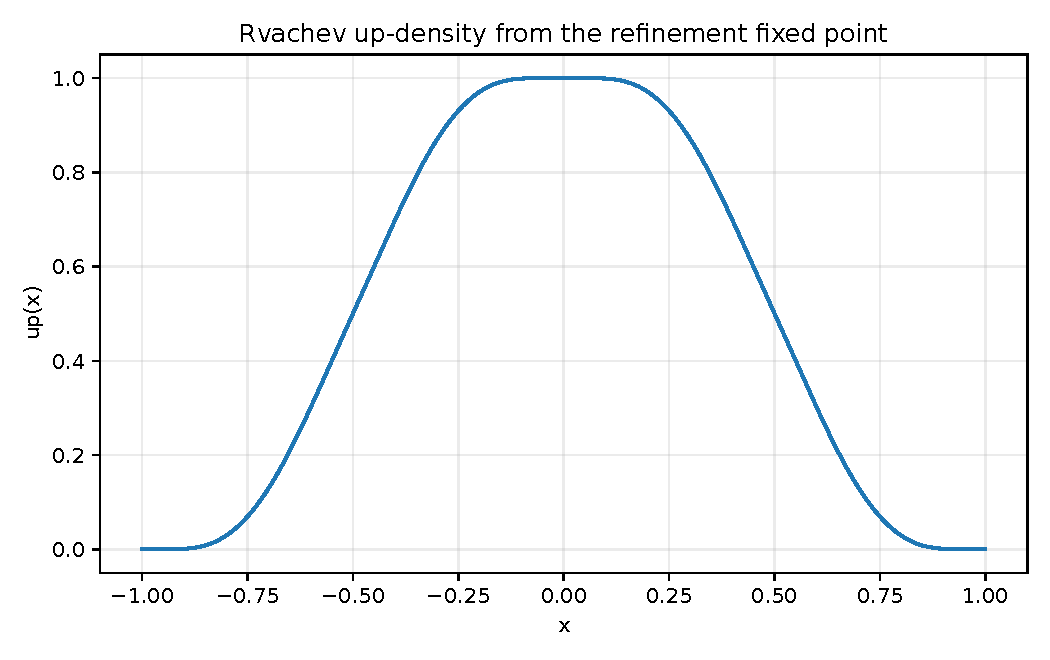
\includegraphics[width=0.82\textwidth]{up_density.pdf}
\caption{The Rvachev density obtained from the refinement fixed point.  The graph
looks rounded at the mode, although every positive-order derivative there is
zero.}
\label{fig:density}
\end{figure}

\begin{figure}[htbp]
\centering
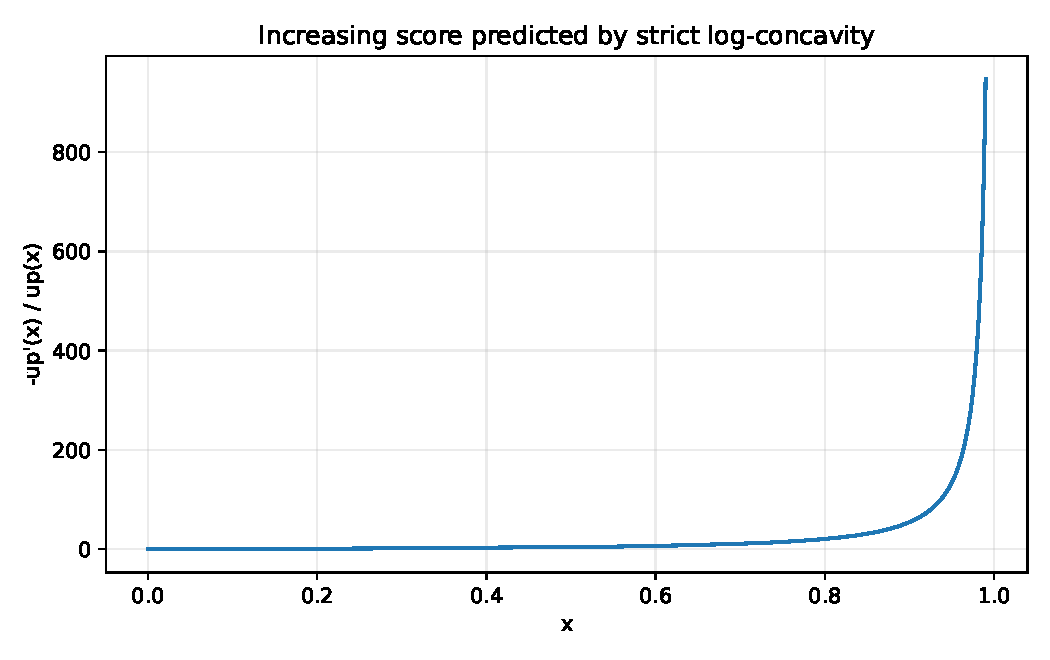
\includegraphics[width=0.82\textwidth]{score_monotonicity.pdf}
\caption{The score $-p'/p$, equivalently the Fabius hazard.  The strict increase
is proved in \cref{thm:hazard}; the plot is a diagnostic rather than evidence used
in the proof.}
\label{fig:score}
\end{figure}

\begin{figure}[htbp]
\centering
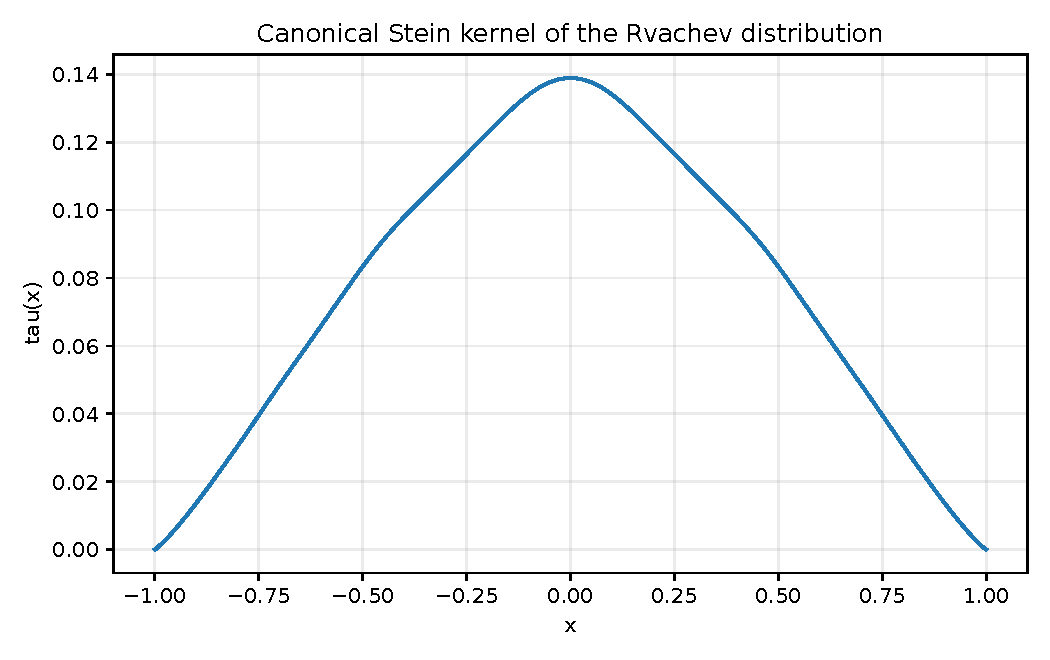
\includegraphics[width=0.82\textwidth]{stein_kernel.pdf}
\caption{The even canonical Stein kernel.  It has exact value $5/36$ at the mode,
a quadratic infinite jet there, and a flat nonanalytic correction that keeps it
positive until the endpoints.}
\label{fig:stein}
\end{figure}

\begin{table}[htbp]
\centering
\caption{Selected fixed-point values.  The score column is simultaneously
$-p'(x)/p(x)$ and the Fabius hazard $F'(x)/(1-F(x))$.}
\label{tab:pointwise}
\begin{tabular}{rrrr}
\toprule
$x$ & $p(x)$ & $\tau(x)$ & score/hazard\\
\midrule
$0$    & $1.0000000000$ & $0.1388888889$ & $0$\\
$0.10$ & $0.9989165644$ & $0.1340355216$ & $0.0589203571$\\
$0.25$ & $0.9305555555$ & $0.1164562604$ & $1.0746268657$\\
$0.50$ & $0.5000000000$ & $0.08333333335$& $4.0000000000$\\
$0.75$ & $0.06944444447$& $0.03948611121$& $14.399999995$\\
$0.90$ & $0.001083435626$&$0.01363282866$& $54.32396650$\\
$0.95$ & $1.6184133\times10^{-5}$&$0.006038886046$&$133.8886201$\\
$0.99$ & $3.5395904\times10^{-11}$&$0.000931860552$&$947.5265981$\\
\bottomrule
\end{tabular}
\end{table}

The exact density values $p(1/4)=67/72$ and $p(3/4)=5/72$ explain the exact
scores $72/67$ and $72/5$ visible in the table.

\section{Endpoint diagnostic}
\begin{figure}[htbp]
\centering
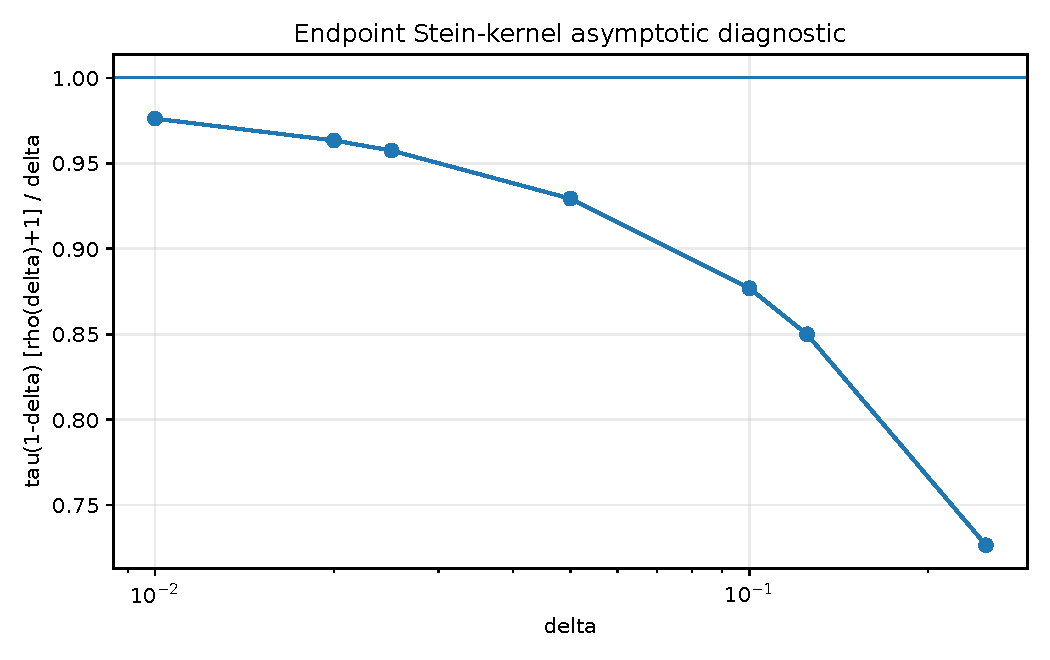
\includegraphics[width=0.82\textwidth]{endpoint_stein_ratio.pdf}
\caption{The ratio predicted to converge to $1$ in
\cref{conj:stein-endpoint}.  The horizontal line is the conjectural limit.}
\label{fig:endpoint-ratio}
\end{figure}

\begin{table}[htbp]
\centering
\caption{Endpoint Stein diagnostic.  Here
$\rho(\delta)=\delta F'(\delta)/F(\delta)$.}
\label{tab:endpoint-numerics}
\begin{tabular}{rrrr}
\toprule
$\delta$ & $\tau(1-\delta)$ & $\rho(\delta)$ &
$\tau(1-\delta)(\rho+1)/\delta$\\
\midrule
$0.250$ & $0.03948611121$ & $3.599999999$ & $0.7265444461$\\
$0.125$ & $0.01770833366$ & $4.999999986$ & $0.8500000136$\\
$0.100$ & $0.01363282866$ & $5.432396650$ & $0.8769176141$\\
$0.050$ & $0.006038886046$& $6.694431004$ & $0.9293158404$\\
$0.025$ & $0.002686175194$& $7.911197165$ & $0.9574814708$\\
$0.020$ & $0.002072559716$& $8.296524734$ & $0.9633801332$\\
$0.010$ & $0.000931860552$& $9.475265981$ & $0.9761487140$\\
\bottomrule
\end{tabular}
\end{table}

The second normalization $\tau(1-\delta)\rho(\delta)/\delta$ rises from about
$0.569$ at $\delta=1/4$ to $0.883$ at $\delta=10^{-2}$, also consistent with the
weaker equivalent in \eqref{eq:stein-endpoint-conj}.  Grid interpolation becomes
unreliable much below $\delta=10^{-2}$ because the density is already extremely
small; endpoint asymptotic evaluation should replace brute-force gridding there.

\section{Stein discrepancy from Gaussianity}
For the centered Gaussian with the same variance, the Stein kernel is the constant
$\sigma^2=1/9$.  The computation gives
\begin{equation}\label{eq:stein-discrepancy-numeric}
 \E\tau(Z)^2\approx0.0129205621965,
\end{equation}
and therefore the dimensionless quadratic Stein discrepancy
\begin{equation}\label{eq:normalized-stein-discrepancy}
 \frac{\E(\tau(Z)-1/9)^2}{(1/9)^2}
 =81\Var(\tau(Z))
 \approx0.04656553792.
\end{equation}
This number is not claimed exact.  Obtaining a closed $q$-series or dyadic-integral
form for it is one of the concrete problems proposed below.

\section{A monotonicity conjecture suggested by the data}
The exact ODE can be written
\begin{equation}\label{eq:tau-hazard-ode}
 \tau'(x)=h_X(x)\tau(x)-x,
 \qquad 0<x<1.
\end{equation}
All sampled derivatives are negative, but strict decrease does not follow from
ordinary log-concavity alone.

\begin{conjecture}[Stein-kernel unimodality]\label{conj:tau-monotone}
The Stein kernel $\tau$ is strictly decreasing on $[0,1)$ and strictly increasing
on $(-1,0]$.  Equivalently,
\begin{equation}
 h_X(x)\tau(x)<x,
 \qquad 0<x<1.
\end{equation}
\end{conjecture}
\Status{\Conjectural; numerically verified on the reported grid}

The kernel is not globally concave on $[0,1)$; numerical second derivatives change
sign.  Thus monotonicity, rather than concavity, is the plausible sharp shape
statement.

\chapter{Conjecture register and frontier program}

\section{Strictness for the full connected-support family}
The geometric densities $h_a$ from \eqref{eq:Za} are known in the repository to
be log-concave for $1<a\le2$, while strict log-concavity is conjectured.  The proof
of \cref{thm:strict-logconcave} reduces the binary endpoint to a no-exponential-
patch theorem.  This suggests the following sharpened formulation.

\begin{conjecture}[Strict geometric-family log-concavity]\label{conj:strict-a}
For every $1<a\le2$, the density $h_a$ is strictly log-concave on $(-1,1)$.
Equivalently, no $h_a$ agrees with $Ce^{bx}$ on a nonempty interval.
\end{conjecture}

A promising proof strategy is to insert a hypothetical exponential patch into the
$a$-refinement equation.  Differentiating propagates the patch through affine
preimages.  For $1<a<2$ those preimages overlap; one expects either a dense family
of exponential patches or a finite-dimensional exponential-polynomial closure,
both incompatible with compact support.  This route needs less than full nowhere
analyticity and may therefore work uniformly in $a$.

\section{Factor divisors and Thue--Morse automata}
\Cref{conj:factor-rigidity} asks whether every compact factor is obtained by
selecting entries of the Bernoulli triangle \eqref{eq:bernoulli-triangle}.  Three
intermediate problems are more approachable.

\begin{problem}[Finite-level divisor classification]
Classify all factorizations into characteristic polynomials of
\[
 \Phi_N(\xi)=\prod_{m=1}^{N}\cos\!\left(\frac{\pi\xi}{2^m}\right)^m.
\]
Can positive definiteness be recognized by a finite Thue--Morse automaton on the
zero allocations?
\end{problem}

\begin{problem}[Uniform indecomposable atoms]
Describe all compact probability factorizations of a single sinc factor after
iterating Vieta's identity.  Determine whether every factor is a Bernoulli digit
subproduct times a translation.
\end{problem}

\begin{problem}[Entire quotient positivity]
Given an integer-valued zero divisor bounded by $1+\nu_2(m)$, characterize when
the corresponding canonical product is positive definite on $\R$.
\end{problem}

A solution would connect harmonic analysis, entire functions of exponential type,
and the arithmetic of the Thue--Morse cosine products.

\section{Stein arithmetic}
\Cref{cor:tau-dyadic} gives rationality but not denominator structure.  Define
\[
 T_{n,k}=\tau\!\left(\frac{k}{2^n}\right),
 \qquad |k|<2^n.
\]
Natural questions include:

\begin{enumerate}
\item exact $2$-adic valuations of $T_{n,k}$;
\item common denominators across a dyadic mesh;
\item recurrences coupling $T_{n,k}$ to the repository's moment integers and
Reshetnikov numbers;
\item a Bell-polynomial formula for Taylor jets of $\tau$ at arbitrary dyadic
points;
\item closed forms for $\E\tau(Z)^m$ and in particular the discrepancy
\eqref{eq:normalized-stein-discrepancy}.
\end{enumerate}

The quotient form $\tau=A/p$ indicates that denominator cancellation should be
substantial.  The half-point rational shadow \eqref{eq:tau-half-rational} suggests
that local jets may have simpler arithmetic than either numerator or denominator
separately.

\section{Stein spectral theory and Legendre comparison}
The divergence-form eigenproblem is
\begin{equation}\label{eq:sturm-liouville}
 -(\tau p g')'=\lambda p g,
 \qquad -1<x<1,
\end{equation}
with natural zero-flux behavior at the endpoints.  The following program would
connect the new operator directly to the repository's Legendre expansions.

\begin{enumerate}
\item Prove closability and compactness of the Dirichlet form
$\mathcal E(g,g)=\int\tau g'^2p$ and obtain a simple discrete spectrum
$0=\lambda_0<\lambda_1=1<\lambda_2<\cdots$ with alternating parity.
\item Establish a singular Sturm--Liouville Weyl law.  The Liouville length is
expected to be
\[
 \mathscr L=\int_{-1}^1\frac{dx}{\sqrt{\tau(x)}},
\]
with $\lambda_n\sim(\pi n/\mathscr L)^2$ if the endpoint classification permits
the standard law.
\item For each eigenfunction, compute the flat correction to its Legendre jet.
At the triangular formal values $n(n+1)/2$, quantify the residual
$r(x)P_n''(\sqrt{18/5}\,x)$.
\item Expand the true eigenfunctions in the even/odd Legendre bases already
developed in the repository and determine whether the coefficient matrix has
hidden total positivity or dyadic arithmetic.
\item Compare the semigroup generated by \eqref{eq:sde} with the Ornstein--Uhlenbeck
semigroup.  The exact normalized Stein discrepancy is a natural first perturbative
parameter.
\end{enumerate}

\begin{conjecture}[Flat Legendre correction principle]
For every eigenvalue $\lambda$ of the closed Rvachev--Stein operator, an
eigenfunction of fixed parity equals the corresponding analytic local Legendre
solution plus a nonzero function flat at $0$.  For $\lambda\ne0,1$, the flat
correction is unavoidable and determines the global boundary quantization.
\end{conjecture}

\section{Endpoint completion}
The exact formula \eqref{eq:log-coordinate} reduces Stein endpoint asymptotics to
control of $\rho$ on a logarithmic window of width $O(1/\rho)$.  The repository's
all-orders Fabius endpoint expansions should permit the following sequence.

\begin{enumerate}
\item Insert the Lambert--$W$ carrier for $F$ into
$\rho=\delta(\log F)'$ and prove a uniform slow-variation lemma.
\item Derive \cref{conj:stein-endpoint} with an explicit relative error, ideally
$O(1/\rho)$.
\item Transfer the bounded dyadic-periodic phase to $\tau$ and identify the first
phase-dependent coefficient.
\item Feed the result into the Liouville length and endpoint classification for
\eqref{eq:sturm-liouville}.
\item Determine whether geometric concavity
\cref{conj:geometric-concavity} follows directly from the saddle representation.
\end{enumerate}

\section{Inverse-function consequences}
Strict log-convexity of $I'$ can be used algorithmically.  On each side of $1/2$,
$\log I'$ has monotone derivative, so tangent and secant bounds give certified
multiplicative envelopes for the inverse slope.  Combined with the existing
Lambert--$W$ endpoint seeds, this suggests globally certified Newton or Halley
schemes whose step acceptance is controlled by log-convexity rather than by crude
interval arithmetic.

A further analytic problem is to classify the higher logarithmic derivatives of
$I'$.  The first nontrivial inequality is \eqref{eq:inverse-third}; possible
higher-order total positivity would connect the inverse Fabius function to
Pick/Stieltjes or generalized Bernstein classes, though no such membership is
asserted here.

\chapter{A Lean-oriented formalization blueprint}

\section{Dependency graph}
The new theory can be formalized in layers that reuse the existing Fabius Lean
walkthrough.

\subsection*{Layer 1: imported analytic object}
Formalize or import:
\begin{enumerate}
\item positivity and smoothness of $p$ on $(-1,1)$;
\item compact support, evenness, and the refinement equation;
\item log-concavity of $p$;
\item the theorem that $p$ is analytic on no open subinterval.
\end{enumerate}

\subsection*{Layer 2: strict shape}
Add general library lemmas:
\begin{enumerate}
\item equality at one interior point of a concave chord implies affinity on the
whole chord;
\item a positive function with affine logarithm is analytic;
\item strict log-concavity implies strict decrease of the logarithmic derivative;
\item Prekopa specialization for moving half-lines, or a one-dimensional proof of
CDF log-concavity.
\end{enumerate}
Then \cref{thm:strict-logconcave,thm:cdf-survival,thm:hazard} become short
compositions.

\subsection*{Layer 3: entire-zero obstruction}
Formalize:
\begin{enumerate}
\item compact support of an identical convolution root;
\item entire extension of compactly supported characteristic functions;
\item multiplicativity of zero order under powers;
\item the simple zero of the first sinc factor.
\end{enumerate}
The proof of \cref{thm:rootless} then has essentially four lines.

\subsection*{Layer 4: Stein kernel}
Define
\[
 A(x)=\int_x^1tp(t)\,dt,
 \qquad \tau(x)=A(x)/p(x).
\]
Prove differentiation, evenness, integration by parts, and the Fabius-tail change
of variables.  The conditional formula can be formalized without conditional
expectation by first proving its numerator/denominator integral identity.

\subsection*{Layer 5: jets and Legendre shadow}
A convenient abstraction is the ideal of functions flat at a point.  Prove that
it is closed under sums, products, composition with smooth functions, and division
by a nonvanishing smooth germ.  Then:
\begin{enumerate}
\item $p-1$ is flat at $0$;
\item $\tau-(5/36-x^2/2)$ is flat;
\item the eigen-equation descends modulo the flat ideal to the Legendre equation;
\item analyticity of $\tau$ on an interval would imply analyticity of $p$ by the
first-order ODE.
\end{enumerate}
This quotient-by-flat-functions viewpoint is cleaner than proving every derivative
identity separately.

\section{Suggested theorem names}
A possible Lean namespace could include:
\begin{lstlisting}
Fabius.up_strictLogConcave
Fabius.cdf_strictLogConcave
Fabius.hazard_strictMono
Fabius.inverse_deriv_strictLogConvex
Fabius.upLaw_no_convolutionPowerRoot
Fabius.steinKernel_eq_tailIntegral
Fabius.steinKernel_zero
Fabius.steinKernel_half
Fabius.stein_weightedPoincare_sharp
Fabius.steinKernel_flatGerm
Fabius.steinEigen_jet_legendre
Fabius.steinEigen_analytic_rigidity
\end{lstlisting}

\section{Formalization risk ledger}
The highest-risk imported item is nowhere analyticity on every interior interval.
If that theorem is not yet available in Lean, strict log-concavity can be isolated
as a theorem conditional on a weaker no-exponential-patch hypothesis.  The next
risk is a general Prekopa theorem; for this one-dimensional setting, an elementary
proof through monotone likelihood ratios may be shorter.  The Stein integration
identities and zero-multiplicity obstruction are comparatively low risk.

\chapter{Conclusions}
The principal gain of this report is a new organizing structure rather than one
more isolated formula.  The binary Fabius--Rvachev law is simultaneously:

\begin{itemize}
\item strictly log-concave but infinitely flat at its mode;
\item a law whose density score is exactly the hazard of its own affine CDF;
\item infinitely decomposable into unequal digits but power-rootless under
identical convolution;
\item equipped with a canonical Stein kernel having exact dyadic arithmetic and a
sharp weighted spectral gap;
\item governed locally by an exact Legendre jet while global nonanalyticity forbids
higher analytic eigenfunctions;
\item linked at the endpoint to the same Lambert--$W$ and dyadic-periodic scales
that govern the existing Fabius asymptotic theory.
\end{itemize}

These features are not independent.  Nowhere analyticity upgrades log-concavity to
strictness; strictness controls the hazard; the hazard enters the Stein ODE; the
Stein kernel defines a diffusion; its flat jet produces the Legendre equation; and
its endpoint integral transfers the Lambert scale.  The resulting chain offers a
compact frontier program with proof-sized intermediate goals, exact arithmetic
checks, numerical diagnostics, and a realistic Lean dependency graph.

\appendix

\chapter{Proof supplement: standard log-concavity facts}

\section{Convolution and weak limits}
A uniform density on an interval is log-concave in the extended-value sense.
Finite convolutions of log-concave functions are log-concave by Prekopa's theorem.
The finite partial sums in \eqref{eq:Zseries} therefore have log-concave densities.
Their weak limit has density $p$, and the pointwise/weak closure theorem for
log-concave laws preserves log-concavity.  This is the conceptual proof imported
from the repository's geometric-family volume.

\section{Half-line marginals}
For completeness, write
\[
 H(x)=\int_{\R}\mathbf 1_{\{t\le x\}}p(t)\,dt.
\]
The set $\{(x,t):t\le x\}$ is convex, so its indicator is log-concave in the
extended-value convention.  The product with $p(t)$ is log-concave in $(x,t)$.
Prekopa's theorem shows that the $t$-marginal $H(x)$ is log-concave.  The same
argument with $t\ge x$ treats the survival function.

\section{Derivative monotonicity}
If a differentiable concave function $g$ has $g'(x)=g'(y)$ for $x<y$, monotonicity
of $g'$ forces $g'$ to be constant on $[x,y]$, so $g$ is affine there.  Thus the
derivative of a differentiable strictly concave function is strictly decreasing.
This is the only strictness input needed for the score and likelihood-ratio
results.

\chapter{Proof supplement: Fourier multiplicities}
At an integer $m\ne0$, the $n$th factor in \eqref{eq:sinc-product} vanishes if and
only if $m/2^n$ is a nonzero integer.  This holds exactly for
$0\le n\le\nu_2(m)$.  Each zero is simple because $\sin z$ has simple zeros at
nonzero integer multiples of $\pi$, and the nonvanishing denominator does not
change the order.  The local product therefore has zero order $1+\nu_2(m)$.

The Bernoulli triangle follows by counting pairs $(n,j)$ with $n\ge0$, $j\ge1$,
and $n+j=m$: there are exactly $m$ such pairs.  The support check is
\[
 \sum_{m=1}^{\infty}\frac{m}{2^{m+1}}=1.
\]

\chapter{Numerical file guide}
The archive contains the following reproducibility files.

\begin{longtable}{>{\raggedright\arraybackslash}p{0.34\textwidth}p{0.56\textwidth}}
\toprule
File & Purpose\\
\midrule
\endfirsthead
\toprule
File & Purpose\\
\midrule
\endhead
\path{rvachev_frontier_experiments.py} & Fully commented fixed-point,
derivative, Stein-kernel, CSV, and plotting code.\\
\path{numerical_output/pointwise_values.csv} & Values used in
\cref{tab:pointwise}.\\
\path{numerical_output/endpoint_diagnostics.csv} & Values used in
\cref{tab:endpoint-numerics}.\\
\path{numerical_output/global_diagnostics_readable.txt} & Mass, symmetry,
exact-value checks, log-concavity defect, monotonicity diagnostic, and Stein
discrepancy.\\
\path{numerical_output/*.pdf} & Vector figures embedded in this report.\\
\bottomrule
\end{longtable}

To reproduce the outputs, run
\begin{lstlisting}
python rvachev_frontier_experiments.py --output-dir numerical_output
\end{lstlisting}
from the source directory.  The default computation uses NumPy and Matplotlib.

\chapter{Corpus map used for the audit}
The most important active families encountered in the recursive documentation
tree were:

\begin{enumerate}
\item \texttt{Fabius\_Function\_and\_Rvachev\_Up}: primary exposition and its
probability, Fourier, arithmetic, asymptotic, inverse, and special-function layers;
\item \texttt{FabiusFunction\_Mathematical\_Glossary};
\item \texttt{Non\_Elementarity\_of\_the\_Fabius\_Function};
\item \texttt{fabius\_lean\_walkthrough};
\item \texttt{archive/}: early notes, primary exposition versions, supplements,
$q$-calculus, standalone studies, glossary, Lean, and frontier snapshots;
\item \texttt{papers/}: Arias de Reyna, Haugland, Thue--Morse/lacunary-product,
and related source papers;
\item \texttt{semi-formalized-research-frontiers/drafts/}: Fourier decay,
Thue--Morse, exponents and $q$-series, Lambert $W$, spectra and arithmetic,
integration and transforms, inverse and sampling, representations, polynomial
synthesis, and the 2026 Lagrange/Legendre loop reports;
\item \texttt{non-formalized-research-frontiers/}: exploratory counterparts and
historical frontier material.
\end{enumerate}

The manifest itself states that consolidated documents absorb earlier drafts and
preserve provenance hashes.  The audit therefore treated the consolidated source
as controlling whenever the older source was explicitly described as absorbed
verbatim or editorially deduplicated.

\backmatter

\begin{thebibliography}{99}

\bibitem{repo}
V. Reshetnikov,
\emph{ProveIt: Analysis/FabiusFunction/docs}, public GitHub repository,
\url{https://github.com/VladimirReshetnikov/ProveIt/tree/main/Analysis/FabiusFunction/docs},
accessed August 30, 2026.

\bibitem{manifest}
V. Reshetnikov,
\emph{Draft manifest for the Fabius--Rvachev semi-formalized research frontiers},
\url{https://github.com/VladimirReshetnikov/ProveIt/blob/main/Analysis/FabiusFunction/docs/semi-formalized-research-frontiers/drafts/MANIFEST.md},
accessed August 30, 2026.

\bibitem{arias1982}
J. Arias de Reyna,
\emph{An infinitely differentiable function with compact support: Definition and properties},
Rev. Real Acad. Ciencias Madrid 76 (1982), 21--38; English translation,
arXiv:1702.05442.

\bibitem{arias2018}
J. Arias de Reyna,
\emph{Arithmetic of the Fabius function},
Integers 18 (2018), Paper A51; arXiv:1702.06487.

\bibitem{haugland}
J. K. Haugland,
\emph{Evaluating the Fabius function},
arXiv:1609.07999.

\bibitem{aistleitner}
C. Aistleitner, R. Hofer, and G. Larcher,
\emph{On parametric Thue--Morse sequences and lacunary trigonometric products},
Ann. Inst. Fourier 67 (2017), 637--687; arXiv:1502.06738.

\bibitem{samworth}
R. J. Samworth,
\emph{Recent progress in log-concave density estimation},
Statistical Science 33 (2018), 493--509.

\bibitem{saumardwellner}
A. Saumard and J. A. Wellner,
\emph{Log-concavity and strong log-concavity: a review},
Statistics Surveys 8 (2014), 45--114.

\bibitem{saumard}
A. Saumard,
\emph{Weighted Poincare inequalities, concentration inequalities and tail bounds
related to Stein kernels in dimension one},
Bernoulli 25 (2019), no. 4B, 3978--4006; arXiv:1804.03926.

\bibitem{courtade}
T. A. Courtade, M. Fathi, and A. Pananjady,
\emph{Existence of Stein kernels under a spectral gap, and discrepancy bounds},
Ann. Inst. Henri Poincare Probab. Stat. 55 (2019), 777--790.

\bibitem{fathi}
M. Fathi,
\emph{Stein kernels and moment maps},
Annals of Probability 47 (2019), 2172--2185; updated arXiv:1804.04699.

\bibitem{prekopa}
A. Prekopa,
\emph{Logarithmic concave measures with applications to stochastic programming},
Acta Scientiarum Mathematicarum (Szeged) 32 (1971), 301--316.

\end{thebibliography}

\end{document}
